\section{Tutorial -- Using a Remote Turbine Instance}\label{tutorial.fs.remote.turbine}

A remote Turbine instance may be used instead of TurbineLite. TurbineLite, used by default, runs simulations (e.g., Aspen Plus) on the user's local machine. The remote Turbine gateway has several potential advantages over TurbineLite, while the main disadvantage is the effort required for installation and configuration. Some reasons to run a remote Turbine instance are:
\begin{itemize}
	\item Simulations can be run in parallel.  The Turbine gateway can distribute simulations to multiple machines configured to run FOQUS flowsheet consumers.  FOQUS consumers are basically additional instances of FOQUS running on remote systems which can run a FOQUS flowsheet.
	\item Simulations can be run on machines other than the user's, so as not to tie-up the user's machine running simulations. 
\end{itemize}

The steps below demonstrate how to set up FOQUS to run flowsheets remotely (see Figure \ref{fig.remote.settings}).

\begin{enumerate}
\item Obtain a user name, password, and URL from the site's Turbine administrator.
\item Open FOQUS.
\item Click \bu{Settings} at the top right of the Home window (Figure \ref{fig.remote.settings1}).
\item Select ``Remote'' from the \bu{FOQUS Flowsheet Run Method} drop-down list.
\item Click the \bu{Turbine} tab; this displays the Turbine settings shown in Figure \ref{fig.remote.settings}.
\end{enumerate}

\begin{figure}[H]
	\begin{center}
		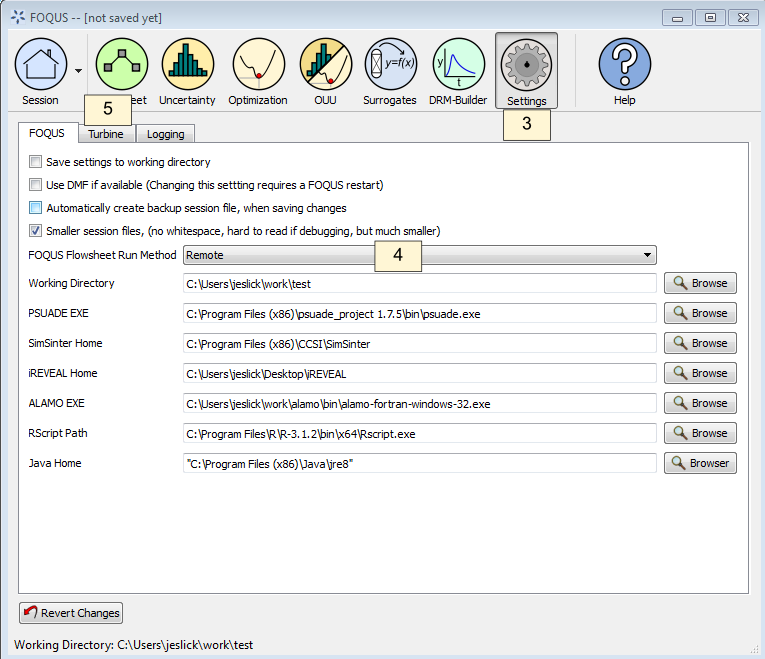
\includegraphics[scale=0.55]{Chapt_flowsheet/figs/settings_turbine_01}
		\caption{Run Method Settings}
		\label{fig.remote.settings1}
	\end{center}
\end{figure}

\begin{enumerate}
\setcounter{enumi}{5}
\item Create a Turbine configuration file; this contains your password in plain text, so it is very important that if you are allowed to choose your own password, you choose one that is not used for any other purpose.
\begin{enumerate}
	\item Click \bu{New/Edit} next to the \textbf{\underline{Turbine Configuration (remote)}} field. The Turbine Configuration window displays (see Figure \ref{fig.remote.settings}).
	\item Select ``Cluster/Cloud'' from the \bu{Turbine Gateway Version} drop-down list in the Turbine Configuration window.
	\item Enter the Turbine URL in the \textbf{\underline{Address}} field.
	\item Enter the \textbf{\underline{User}} name and \textbf{\underline{Password}}.
	\item Click \bu{Save as} and enter a new file name.
	\item Set the remote Turbine configuration file.  Click \bu{Browse} next to the \bu{Turbine Configuration (remote)} field. Select the file created in Step 6e.
\end{enumerate}
\end{enumerate}

\begin{figure}[H]
	\begin{center}
		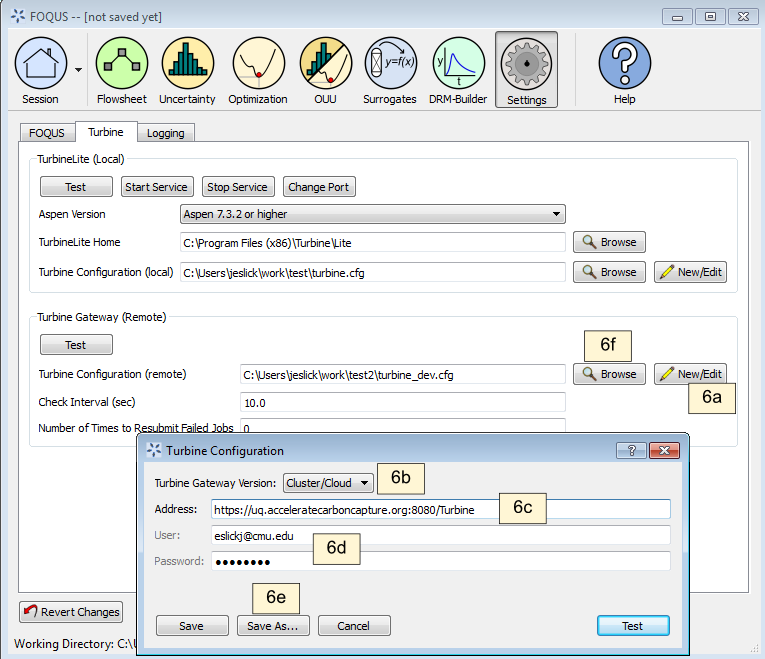
\includegraphics[scale=0.55]{Chapt_flowsheet/figs/remoteSetting}
		\caption{Remote Turbine Settings}
		\label{fig.remote.settings}
	\end{center}
\end{figure}

At this point the remote gateway is ready to use.  The last step is to ensure that all simulations referenced by flowsheets to be run are uploaded to the remote Turbine gateway.

\begin{enumerate}
	\setcounter{enumi}{6}
	\item Upload any necessary simulations to Turbine (see Section \ref{overview.turbine.upload} and the tutorial in Section \ref{tutorial.sim.flowsheet})
\end{enumerate}

Once all settings are specified there is no apparent difference between running flowsheets locally or on a remote Turbine gateway, and FOQUS can readily be switched between the two.
